
\section{Differentialgleichungen}

\subsection{Grundbegriffe}

\begin{description}[labelindent=16pt,style=multiline,leftmargin=3.5cm, noitemsep]
	\item[Ordnung:] h{\"o}chste vorkommende Ableitung
	\item[linear:] alle $y$-abh{\"a}ngigen Terme kommen linear vor (keine Terme wie zum Beispiel $y^2$, $(y'')^3$, $\sin(y)$, $e^{y'}$)
	\item[homogen:] Gleichung ohne St{\"o}rfunktionen
	\item[St{\"o}rfunktion:] Term, der rein von der Funktionsvariablen $x$ abh{\"a}ngt
\end{description}

\subsection{Methoden}

\begin{table}[H]
	\centering
	\begin{tabular}{|p{3cm}|p{6cm}|p{3cm}|}
		\hline
		& \textbf{Problem} 							& \textbf{Anforderungen} 			\\ \hline
		\textbf{Trennung der Variablen}   	& $y' = \frac{dy}{dx} = h(x) \cdot g(y)$ 	& 1. Ordnung			            \\ \hline
		\textbf{Variation der Konstanten}	& $y' = \frac{dy}{dx} = h(x)y + b(x)$	 	& 1. Ordnung \filbreak inhomogen	\\ \hline
		\textbf{Euler-Ansatz}				& $a_{n}y^{(n)} + a_{n-1}y^{(n-1)} + ... + a_{0}y = 0$	 	& n. Ordnung \filbreak linear \filbreak homogen	\\ \hline
		\textbf{Direkter Ansatz}				& $a_{n}y^{(n)} + a_{n-1}y^{(n-1)} + ... + a_{0}y = b(x)$	& n. Ordnung \filbreak linear \filbreak inhomogen	\\ \hline
		
		%\textbf{Substitution}				& $y' = h(\frac{y}{x})$ \filbreak $y' = h(ax + by + c)$ \filbreak $y' = h(\frac{ax + by + c}{dx + ey + f})$ \filbreak $y' = \frac{y}{x}h(xy)$ 																		& nicht direkt separierbar			\\ \hline
	\end{tabular}
\end{table}

\subsubsection{Trennung der Variable}

\begin{equation*}
\begin{split}
& y' + x \tan y = 0,\ y(0) = \frac{\pi}{2} \\
\text{umformen}\quad & \frac{dy}{dx} = -x \tan y \\
\textbf{konstante L{\"o}sungen}\quad & y(x) \equiv 0\ \text{erf{\"u}llt jedoch $y(0) \equiv \frac{\pi}{2}$ nicht} \\
\text{Trennung}\quad & \frac{dy}{\tan y} = -x dx \\
\text{integrieren}\quad & \int\frac{\cos y}{\sin y}dy = - \int xdx \Rightarrow \log|\sin y| = -\frac{x^2}{2} + C \\
& \Rightarrow |\sin y| = e^Ce^{\frac{-x^2}{2}} \Rightarrow \sin y = \pm e^Ce^{\frac{-x^2}{2}} = Ce^{\frac{-x^2}{2}} \\
\text{Anfangsbedingung gebrauchen}\quad & \sin(y(0)) = \sin (\frac{\pi}{2}) = 1 \Rightarrow C = 1 \\
\textbf{L{\"o}sung}\quad & y(x) = \arcsin (e^{\frac{-x^2}{2}})
\end{split}
\end{equation*}



\subsubsection{Variation der Konstanten}

\begin{equation*}
\begin{split}
\textbf{Grundsatz:} &\quad y(x) = y_h(x) + y_p(x) \\
& y'(x+1) + y = x^3,\ y(0) = \sqrt{5} \\
\text{Trennung}\quad & \frac{y'}{y} = \frac{-1}{x+1} \\
\textbf{konstante L{\"o}sungen}\quad & y(x) \equiv 0\ \text{erf{\"u}llt jedoch $y(0) \equiv \sqrt{5}$ nicht} \\
\text{integrieren}\quad & \int \frac{dy}{y} = - \int \frac{dx}{x+1} \\
& \Rightarrow \ln|y| = -\ln|x+1| + C \\
\end{split}
\end{equation*}
\begin{equation*}
\begin{split}
\textbf{Homogene L{\"o}sung} \quad & y_h(x) = \frac{C}{x+1},\ \text{mit}\ C= \pm e^C \in \mathbb{R}\backslash{0} \\
\text{partikul{\"a}rer Ansatz}\quad & y_p(x) = \frac{C(x)}{x+1} \\
\text{einsetzen} \quad & (\frac{C'(x)}{x+1} - \frac{C(x)}{(x+1)^2})(x+1) + \frac{C(x)}{x+1} = x^3 \\
& C'(x) = x^3 \\
& C(x) = \frac{x^4}{4} \\
\textbf{partkul{\"a}re L{\"o}sung} \quad & y_p(x) = \frac{x^4}{4(x+1)} \\
\text{allgemeine L{\"o}sung}\quad & y(x) = y_h(x) + y_p(x) = \frac{C}{x+1} + \frac{x^4}{4(x+1)} \\
\text{Anfangsbedingung benutzen} \quad & y(0) = \sqrt{5} \Rightarrow C = \sqrt{5} \\
\textbf{L{\"o}sung} \quad & y(x) = \frac{\sqrt{5}}{x+1} + \frac{x^4}{4(x+1)}
\end{split}
\end{equation*}

%\subsubsection{Substitution}
%
%\begin{equation*}
%\begin{split}
%	& y' = h(\frac{y}{x})\ \text{ersetzt durch}\ z(x) = \frac{y(x)}{x} \Leftrightarrow y(x) = xz(x) \\
%	& \Rightarrow	y' = z + xz'
%\end{split}
%\end{equation*}



\subsubsection{Euler-Ansatz}

\begin{equation*}
\begin{split}
& y'' - 2y' - 8y = 0,\ y(1) = 1, y'(1) = 0 \\
\text{Euler-Ansatz}\quad & y(x) = e^{\lambda x} \\
\text{einsetzen}\quad & \lambda^2 e^{\lambda x} - 2\lambda e^{\lambda x} - 8e^{\lambda x} = 0 \\
\textbf{charakt. Polynom}\quad & \lambda^2 - 2\lambda - 8 = (\lambda - 4)(\lambda + 2) = 0 \\
\text{Nullstellen}\quad & 4, -2 \\
\textbf{allgemeine L{\"o}sung}\quad & y(x) = Ae^{4x} + Be^{-2x} \\
\text{Anfangsbedingung gebrauchen}\quad & y(1) = Ae^4 + Be^{-2} =1,\\ &y'(1) = 4Ae^4 - 2Be^{-2} = 0 \\
& \Rightarrow A = \frac{1}{3}e^{-4}, B = \frac{2}{3}e^2 \\
\textbf{L{\"o}sung}\quad & y(x) = \frac{1}{3}e^{4x-4} + \frac{2}{3}e^{2-2x}
\end{split}
\end{equation*}

\emph{Bemerkung:} Zu einer $m$-fachen Nullstelle $\lambda$ geh{\"o}ren die $m$ linear unabh{\"a}ngigen L{\"o}sungen $e^{\lambda x}$, $x\cdot e^{\lambda x}$, ... , $x^{m-1}\cdot e^{\lambda x}$. Zur $m$-fachen Nullstelle $\lambda = 0$ geh{\"o}ren die L{\"o}sungen $1$, $x$, ... , $x^{m-1}$. \\

\emph{Komplexe Nullstellen:}


$x = \frac{-b \pm \sqrt{b^2-4ac}}{2a}$


Ein komplexes Nullstellenpaar der Form $\alpha \pm \beta i$ liefert folgende homogene L{\"o}sung:
\begin{equation*}
y(x)=e^{\alpha x}(C_1\cos(\beta x) + C_2\sin(\beta x))
\end{equation*}



\subsubsection{Direkter Ansatz}

\begin{equation*}
\textbf{Grundsatz:}\quad y(x) = y_\text{homo}(x) + y_p(x)
\end{equation*}

\begin{table}[H]
	\centering
	\begin{tabular}{|l|l|l|}
		\hline
		\textbf{Inhomogener Term $b(x)$} & \textbf{Ansatz f{\"u}r $y_p(x)$}	& \textbf{zu bestimmen}		\\ \hline
		Polynom				& $Ax^2 + Bx + C$			& $A$, $B$, $C$		\\ \hline
		$c e^{k x}$ & $Ae^{kx}$					& $A$				\\ \hline
		$c\sin(kx)$ oder $c\cos(kx)$ & $A\sin(kx) + B\cos(kx)$ & $A$, $B$ \\ \hline
		
	\end{tabular}
\end{table}

\emph{Bemerkung:} Kommt der gew{\"a}hlte Ansatz schon in der homogenen L{\"o}sung vor,\\ so multipliziert man den Ansatz einfach mit $x$.

\begin{equation*}
\begin{split}
& y'' - y' + \frac{1}{4}y = \cos(x) \\
\text{homogener Ansatz}\quad & y'' + y' + \frac{1}{4}y = 0 \\
\text{Euler-Ansatz anwenden}\quad & \lambda^2 + \lambda + \frac{1}{4} = (\lambda + \frac{1}{2})^2 = 0 \\
\textbf{homogene L{\"o}sung}\quad &\Rightarrow y_\text{homo}(x) = Ae^{-\frac{x}{2}} + Bx \cdot e^{-\frac{x}{2}} \\
\text{partikul{\"a}rer Ansatz w{\"a}hlen}\quad & y_p(x) = a\cos(x) + b\sin(x) \\
& \Rightarrow y_p'(x) = -a\sin(x) + b\cos(x),\  y_p''(x) = \\ & = -a\cos(x) -b \sin(x) \\
\text{Einsetzen}\quad & (-a + b + \frac{a}{4})\cos(x) + (-b -a + \frac{1}{4}b)\sin(x) \\&= \cos(x) \\
\text{Koeffizientenvergleich}\quad & -\frac{3}{4}a + b = 1,\ -a-\frac{3}{4}b = 0 \\
\end{split}
\end{equation*}

\begin{equation*}
\begin{split}
\textbf{partikul{\"a}re L{\"o}sung}\quad & y_p(x) = -\frac{12}{25}\cos(x) + \frac{16}{25}\sin(x) \\
\textbf{L{\"o}sung}\quad & y(x) = Ae^{-\frac{x}{2}} + Bx \cdot e^{-\frac{x}{2}} -\frac{12}{25}\cos(x) + \frac{16}{25}\sin(x)
\end{split}
\end{equation*}

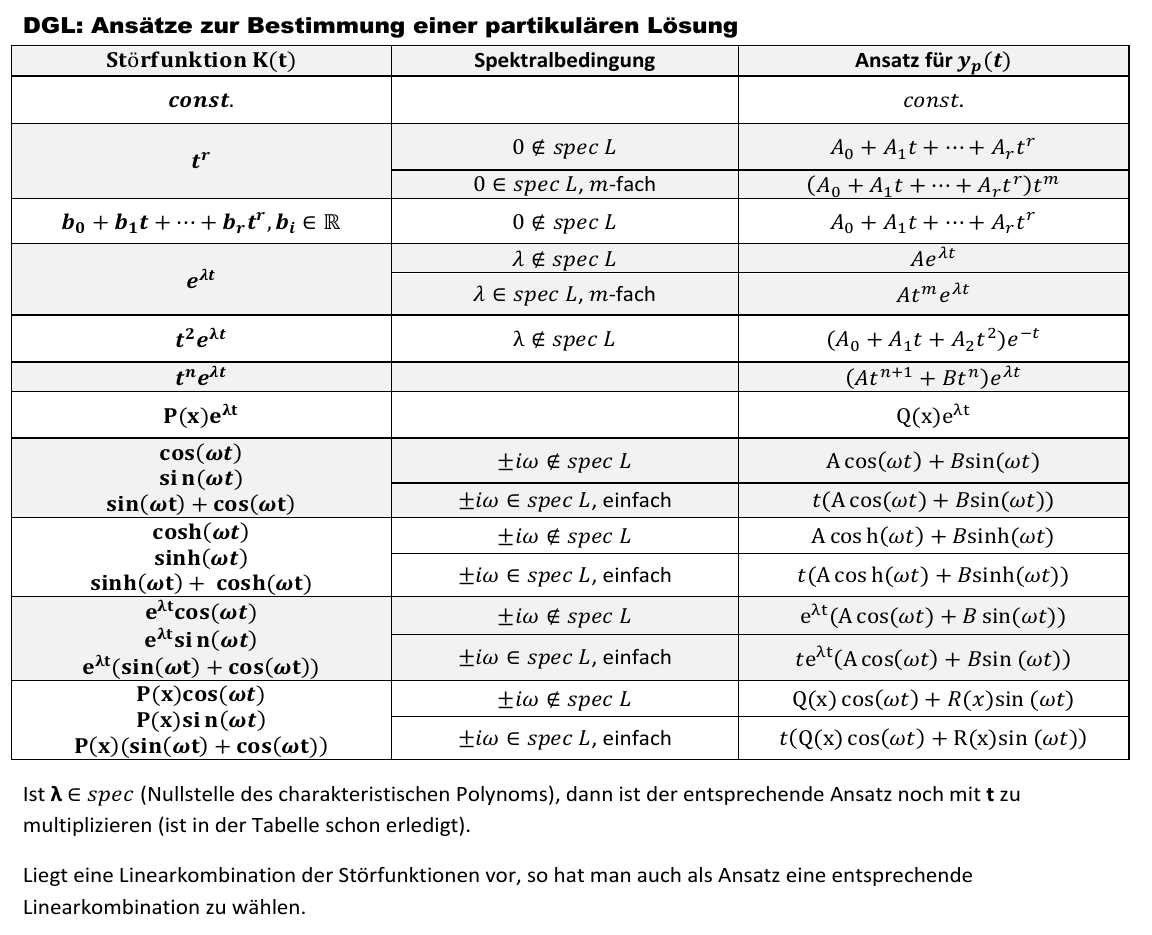
\includegraphics[width=1\textwidth]{images/dgl_ansatze_part_lsg.png}